\chapter{Proposed Heterogeneous CSS Prototype}
\label{chapter5}

This chapter outlines the implementation of heterogeneous test-bed for cooperative spectrum sensing using USRP N210 and RTL-SDR software defined radios. We start with heterogeneous cooperative spectrum sensing, where we first describe the experimental setup, which is implemented using soft and hard fusion schemes. The sensor nodes, which consists of three RTL-SDRs and one USRP N210, are placed in a controlled indoor laboratory environment approximately 8-10 meters apart. The signal source is being simulated by another USRP N210, which is transmitting a DQPSK signal at 450 MHz. The post-processing is done on a Fusion Center (FC), which makes the decision based on global test statistic using both soft and hard decision schemes. Finally, we discuss the results where the performance of both the schemes are evaluated in a real fading scenario on a hardware test-bed. 

\section{Experimental Setup for Proposed Heterogeneous CSS Prototype}

The measurements are performed using software-defined radios (SDRs) and the post-processing is conducted on desktop computers. The desktop computer consists of i7 Intel processor with eight cores and 3.41 GHz clock cycle running Ubuntu 16.04. The sensor node network is implemented using RTL-SDR dongles and Ettus Research USRP N210 on GNU Radio Software platform. The measurements are analyzed in MATLAB and measurement plots are generated. Figure~\ref{expsetup} presents a photograph of the actual proposed prototype system, which consists of three RTL-SDRs and two USRP N210s. One USRP N210 (middle) acts as a primary user while the other SDRs operate as sensor nodes. All the SDRs were placed in a laboratory environment at least 5-6 meters away from the primary user.

\begin{sidewaysfigure}
\centering
	\includegraphics[width=\textwidth]{images/Gill/figs/setup.eps} 
\caption{Experimental Test-Bed For Cooperative Sensing in Heterogeneous Network. Sensors 1, 2 and 4 are RTL-SDR units, sensor 3 is USRP N210 and TX is another USRP N210 unit which is used as a signal source for this work.}
\label{expsetup}
\end{sidewaysfigure}

These sensor nodes collect the spectral data, normalize it, and then transmit it to the FC for the detection. For soft data fusion, the data is quantized in the local sensor nodes before it is transmitted to FC due to the limited bandwidth of the overhead channel. The delays caused by the different sensor nodes is ignored, as it would require extra computational complexity and it is out of the scope of this thesis. The USRP N210 transmits a DQPSK modulated signal with 4 samples per symbol with the alpha factor of the root raised cosine filter set to 0.35. The transmitter gain and amplitude are varied in order to get different SNR values for each node. The sensor nodes collect the data via 300,000 energy samples, and each measurement is conducted three times in order to eliminate any irregularities. The noise variance $\sigma_n^2$ for each SU is estimated by running each sensor node without any transmission at 450 MHz. The flow-graph is executed multiple times to get a better estimate of noise variance. Once the data is received from all the sensor nodes, the Probability of Detection ($P_d$) is calculated for different received SNR values for all the sensor nodes. To properly evaluate the performance of each of the cooperative spectrum sensing techniques, the average $P_d$ is calculated for each scheme. 

All four sensor nodes have different sampling rates to model potential differences existing within a heterogeneous environment. The USRP N210, which is also used as a $4^{th}$ sensor node, has a very low noise floor compared to the three other radios and hence can detect a signal with very low SNR. This is a challenging factor for data fusion when the nodes have different operating parameters and the FC has to make optimal decisions by combining this varying data. Due to their spatial diversity, the node closest to the transmitter will have different SNR compared to the other nodes. All these factors impact the data combining at the FC. The GNU Radio flow-graph for the sensor nodes is shown in the Figure~\ref{receiver}. The same flow-graph is used for all sensor nodes with different operating parameters. For the USRP N210 node, we replaced the RTL-SDR source with UHD:USRP Source gnuradio block. The central frequency is kept at 450 MHz and the operating parameters of each sensor node is provided in Table~\ref{tablehet}. The values of the transmitter amplitude and gain are varied to get the different sets of SNR values which are used for computing $P_d$ values for each node. The plots are generated in MATLAB by using the data files from the GNU Radio platform.

To evaluate the performance of the cooperative spectrum sensing, the USRP N210 is used as a transmitter, where its gain and amplitude are varied. Figure~\ref{transmitter} shows the flow-graph used for the transmitter. The flow-graph starts with the random source block, which generates the random data between zero and three, and passes it to the differential phase shift keying (DPSK) modulator block. The DPSK block modulates the signal with differential quadrature phase shift keying (DQPSK) scheme, applies root raise cosine filter with excess bandwidth value of 0.35, and passes it to a multiply const block. It is used to control the SNR value and finally the data is dumped into the USRP N210 sink, which transmits the data over the air where other sensor nodes can estimate the signal presence using soft and hard decision schemes.

\begin{figure}[ht!]
	\centering
	\includegraphics[width=\textwidth,keepaspectratio]{images/Gill/figs/transmitter.eps}
    \caption{GNU Radio Flowgraph For Transmitter Running on USRP N210.} 
\label{transmitter}      
\end{figure}

\begin{figure}[ht!]
	\centering
	\includegraphics[width=\textwidth,keepaspectratio]{images/Gill/figs/normalizedenergy.eps}
    \caption{GNURadio Flowgraph For USRP and RTL-SDR sensor nodes.} 
\label{receiver}      
\end{figure}

\begin{table}[!ht]
\caption{Operating Characteristics of Sensor Nodes}
\centering
\vspace{-5pt}
\begin{tabular}{c c c c c}
\toprule
Nodes      & $F_s$     & Gain  & FFT Size &  Bin Size \\ \hline
RTL-SDR-1  & 1.1 Msps  & 10 dB & 512      & 2.148 KHz \\ \hline
RTL-SDR-2  & 1.8 Msps  & 10 dB & 512      & 3.515 KHz\\ \hline
RTL-SDR-3  & 2.4 Msps  & 10 dB & 512      & 4.687 KHz\\ \hline
USRP N210  & 7.2 Msps  & 10 dB & 512     &  14.062 KHz\\ 
\bottomrule
\end{tabular}
\vspace{-5pt}
\label{tablehet}
\end{table}

The sensor nodes are placed inside the laboratory and are connected to distributed system. Figure~\ref{receiver} shows the flowgraph running on the receiver, for flow-graph running on USRP we use UHD:USRP source instead of RTL-SDR source. The frequency around 450 MHz is sweeped in regular intervals and the continuous data stream is passed to FFT block, which does the forward FFT operation with a Blackmann Harris window. The data is first converted into parallel stream of the FFT size using stream to vector GNU Radio block. The complex-to-magnitude block converts the complex values into float and take their magnitude. The bin selector block is used to select the bin where the narrowband signal is being transmitted. We then take the moving average of the values, normalize them and then store it to the file sink. The normalized energy values are collected for each sensor at different SNR values and then post processing is performed in MATLAB. The operating parameters of each sensor node is provided in the Table~\ref{tablehet}.

\section{Hard-Data Fusion Scheme}
\label{hardfusion}
Cooperative spectrum sensing using hard-data fusion is a proven method for improving the detection performance. In this scheme, all sensor nodes sense the signal source individually and send their sensing decision in the form of 1-bit binary data. For hard data fusion, the noise $w_q$ can be neglected since the sensor nodes can just transmit their decision statistic in an efficient way, where the floating values are not required. For example, the SUs can just transmit ''1'' and ''0'' depending on whether the primary user is present or absent. Furthermore, in the Fusion Center the decision can be made by using the OR, AND, or majority rule algorithms. For the AND decision rule, the FC performs the logical AND operation for all the local decisions and conducts the detection. Similarly, for the OR rule, the logical OR operation is used to decide whether the signal is present or not. Finally, the majority rule conducts majority vote and decides based on it~\cite{ghasemi2005collaborative,duan2010performance}. The $P_d$ for AND, OR and Majority Rule for $R=4$ sensor nodes is given by~\cite{inphtn15}:
\begin{equation}
P_{d,AND} = (P_d)^4\nonumber\\
\vspace{-15pt}
\end{equation}
\begin{equation}
\label{hard}
~~~~~~~P_{d,OR} = 1-(1-P_d)^4
\vspace{-15pt}
\end{equation}
\begin{equation}
P_{d,MJR} = 6P_{davg}^2(1-P_{davg})^2+4P_{davg}^3(1-P_{davg})+P_{davg}^4\nonumber
\end{equation}
where $P_{davg}$ is the average probability of detection of the sensor units. Similarly, we can calculate the $P_{fa}$ for all three schemes by replacing $P_{davg}$ by $P_{faavg}$ in Eq~(\ref{hard}).

\begin{figure}[ht!]
	\centering
	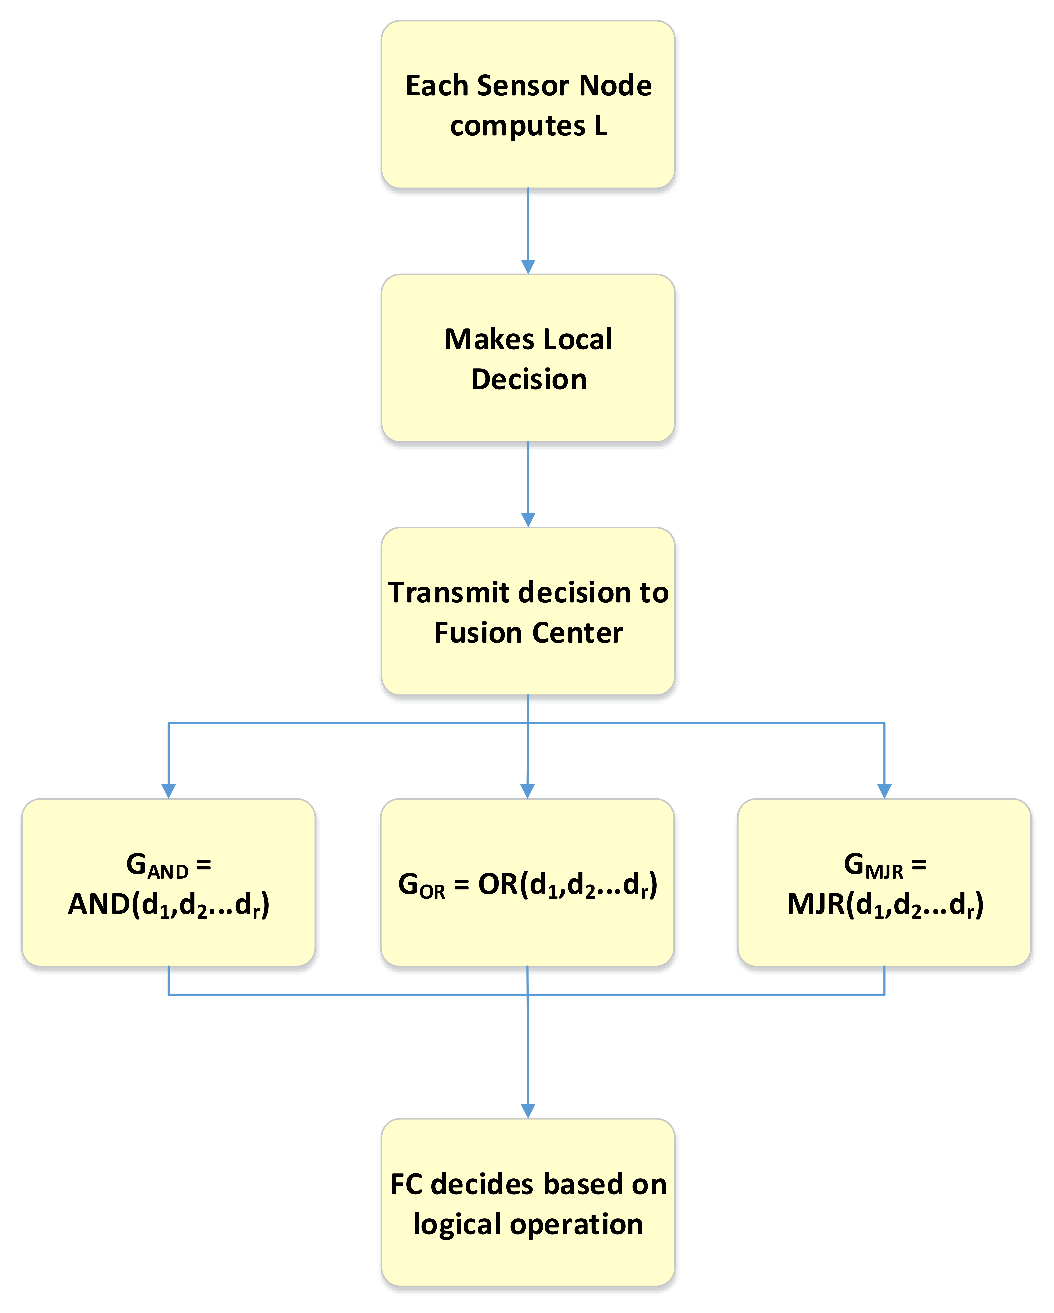
\includegraphics[width=\textwidth,height=10cm,keepaspectratio]{images/Gill/figs/hardfusion.eps}
\caption{Flowchart showing AND, OR and Majority Rule Fusion schemes.} 
\label{hard}      
\end{figure}

\section{Soft-Data Fusion Scheme}

In soft-data fusion based cooperative spectrum sensing, information from different CR users is combined to make a decision on the presence or absence of the primary user. In Section~\ref{hardfusion}, we discussed the conventional hard combination, where each CR user feedbacks one-bit message regarding whether observed energy is above a certain threshold. In this section, we discuss soft combination of the local test statistic of each sensor nodes and how it is combined to make the decision in the FC. Since in the soft combination accurate energy values from different CR users are utilized to make a decision, this scheme is more accurate and complex to implement. In this thesis, we discuss two popular soft decision fusion schemes: \textit{Maximum Normalized Energy} (MNE) scheme and \textit{Equal Gain Combining} (EGC) scheme.

For MNE, the local test statistic in each sensor node is computed and then transmitted to FC after quantization. In this thesis, we are using four sensor nodes equipped with different sensing abilities such as the sampling rates and noise floor. Therefore, the global test statistic $G$ can be modeled by:
\begin{equation}
\label{eq:8}
G_{MNE} = \max\{\beta_r\}.
\end{equation}
The $P_{fa}$ and $P_d$ values for the MNE-CS is given by~\cite{inhtn12}:
\begin{equation}
\label{eq:9}
P_{fa} = 1-\prod_{r=1}^R\Bigg(1-Q\Bigg(\dfrac{\tau-1}{\sqrt{\dfrac{1}{M_r}+\sigma_{q,r}}}\Bigg)\Bigg),
\end{equation}
\begin{equation}
\label{eq:10}
~~~~~~P_d = 1-\prod_{r=1}^R\Bigg(1-Q\Bigg(\dfrac{\tau-1-\gamma_r}{\sqrt{\dfrac{1+2\gamma_r}{M_r}+\sigma_{q,r}}}\Bigg)\Bigg),
\end{equation}
where $\tau$ is the global threshold for MNE, $M_r$ is the number of samples for $r^{th}$ sensor node, and $\sigma_{q,r}$ is the noise variance for the received local test statistic. The algorithm for MNE-CS is illustrated by the flowchart in Figure~\ref{mnescheme}.

\begin{figure}[ht!]
	\centering
	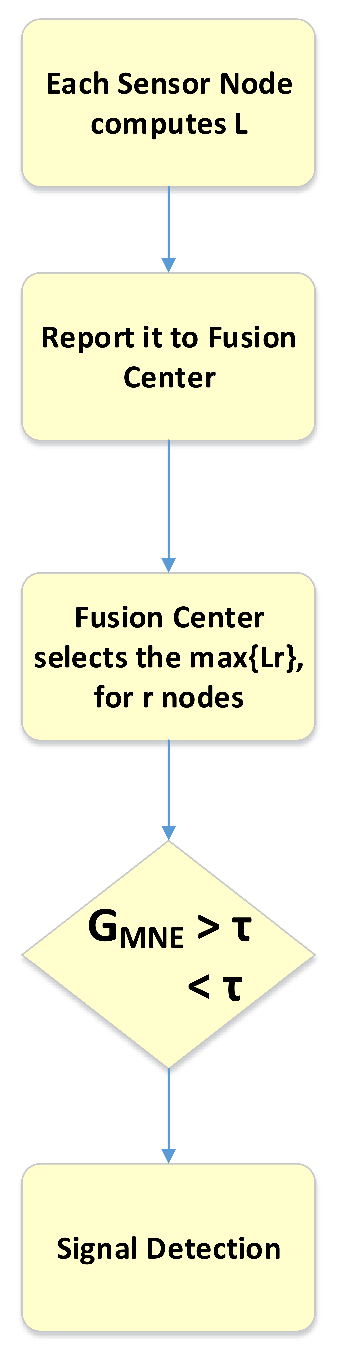
\includegraphics[width=\textwidth,height=10cm,keepaspectratio]{images/Gill/figs/mnescheme.eps}
\caption{Flowchart describing Maximum Normalized Energy Scheme.} 
\label{mnescheme}      
\end{figure}

For EGC, the global decision statistic is the mean of the $\beta$ values for all the sensor nodes. It has been shown in \cite{inhtn12} that the EGC scheme performs better than the MNE scheme in a noisy channel. The EGC scheme can be modeled by:
\begin{equation}
	\label{eq:11}
	 G_{EGC} = \dfrac{1}{M}\sum_{r=1}^{M}{\beta_r},
\end{equation}
where $G_{EGC}$ is global test statistic of EGC scheme. The $P_{fa}$ and $P_d$ values for the EGC-CS scheme are given by:
\begin{equation}
\label{eq:12}
P_{fa} = Q\Bigg(\dfrac{\tau-1}{\sqrt{\dfrac{1}{R^2}\sum_{r=1}^{R}\bigg(\dfrac{1}{M_r}+\sigma_{q,r}^2\bigg)}}\Bigg),
\end{equation}

\begin{equation}
\label{eq:13}
~~~~~~P_d = Q\Bigg(\dfrac{\tau-\dfrac{1}{R}\sum_{r=1}^R(1+\gamma_r)}{\sqrt{\dfrac{1}{R^2}\sum_{r=1}^{R}\bigg(\dfrac{1+2\gamma_r}{M_r}+\sigma_{q,r}^2\bigg)}}\Bigg).
\end{equation}
The algorithm for EGC-CS is also illustrated by the flowchart in Figure~\ref{egcscheme}.

\begin{figure}[ht!]
	\centering
	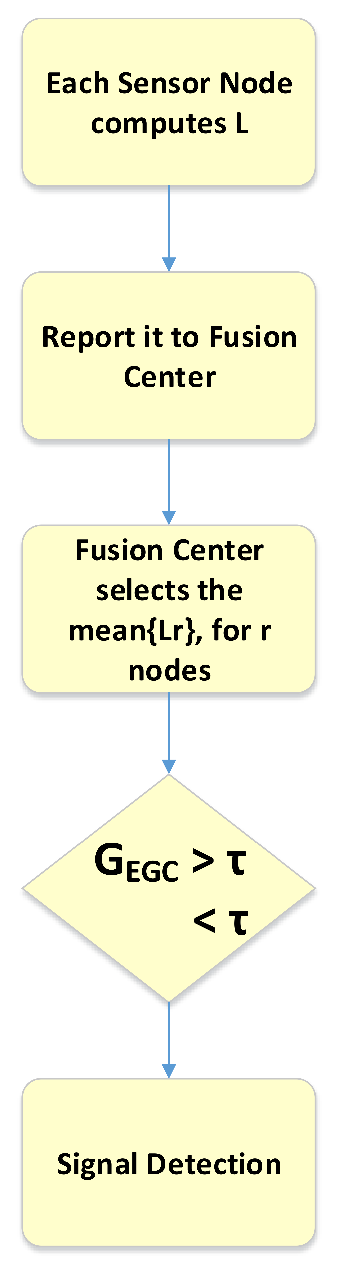
\includegraphics[width=\textwidth,height=10cm,keepaspectratio]{images/Gill/figs/egcscheme.eps}
\caption{Flowchart describing Equal Gain Combining Scheme.} 
\label{egcscheme}      
\end{figure}

\section{Experimental Results}
In this thesis, we implemented the heterogeneous cooperative spectrum sensing (CSS) using both hard and soft data fusion schemes. We start by collecting the data across 450 MHz band for all sensor nodes in a distributed manner. The spectrum sensing data is normalized for both soft and hard data fusion schemes using the same operational parameters to compare their performance accurately. The measurements are performed using software-defined radios (SDRs) and the post processing is conducted on desktop computers. The desktop computer consists of an i7 Intel processor with eight cores and 3.41 GHz clock cycle running Ubuntu 16.04. The sensor node network is implemented using RTL-SDR dongles and Ettus Research USRP N210 on GNU Radio Software platform.
These sensor nodes collect the spectral data, normalize it and then transmit it to the FC for the detection. For soft data fusion, the data is quantized in the local sensor nodes before it is transmitted to FC due to the limited bandwidth of the overhead channel. 

Figure~\ref{hardres} shows the $P_{davg}$ versus $SNR_{avg}$ for all four sensor nodes when hard decision combining is performed. It can be seen that OR performs the best, while AND performs the worst in a fading channel. The SNR average was computed by taking the mean of all the SNRs for the sensor nodes. The SNR was varied for each sensor node by varying the transmitter amplitude and gain in the GNU Radio flow-graph.

\begin{figure}[ht!]
	\centering
	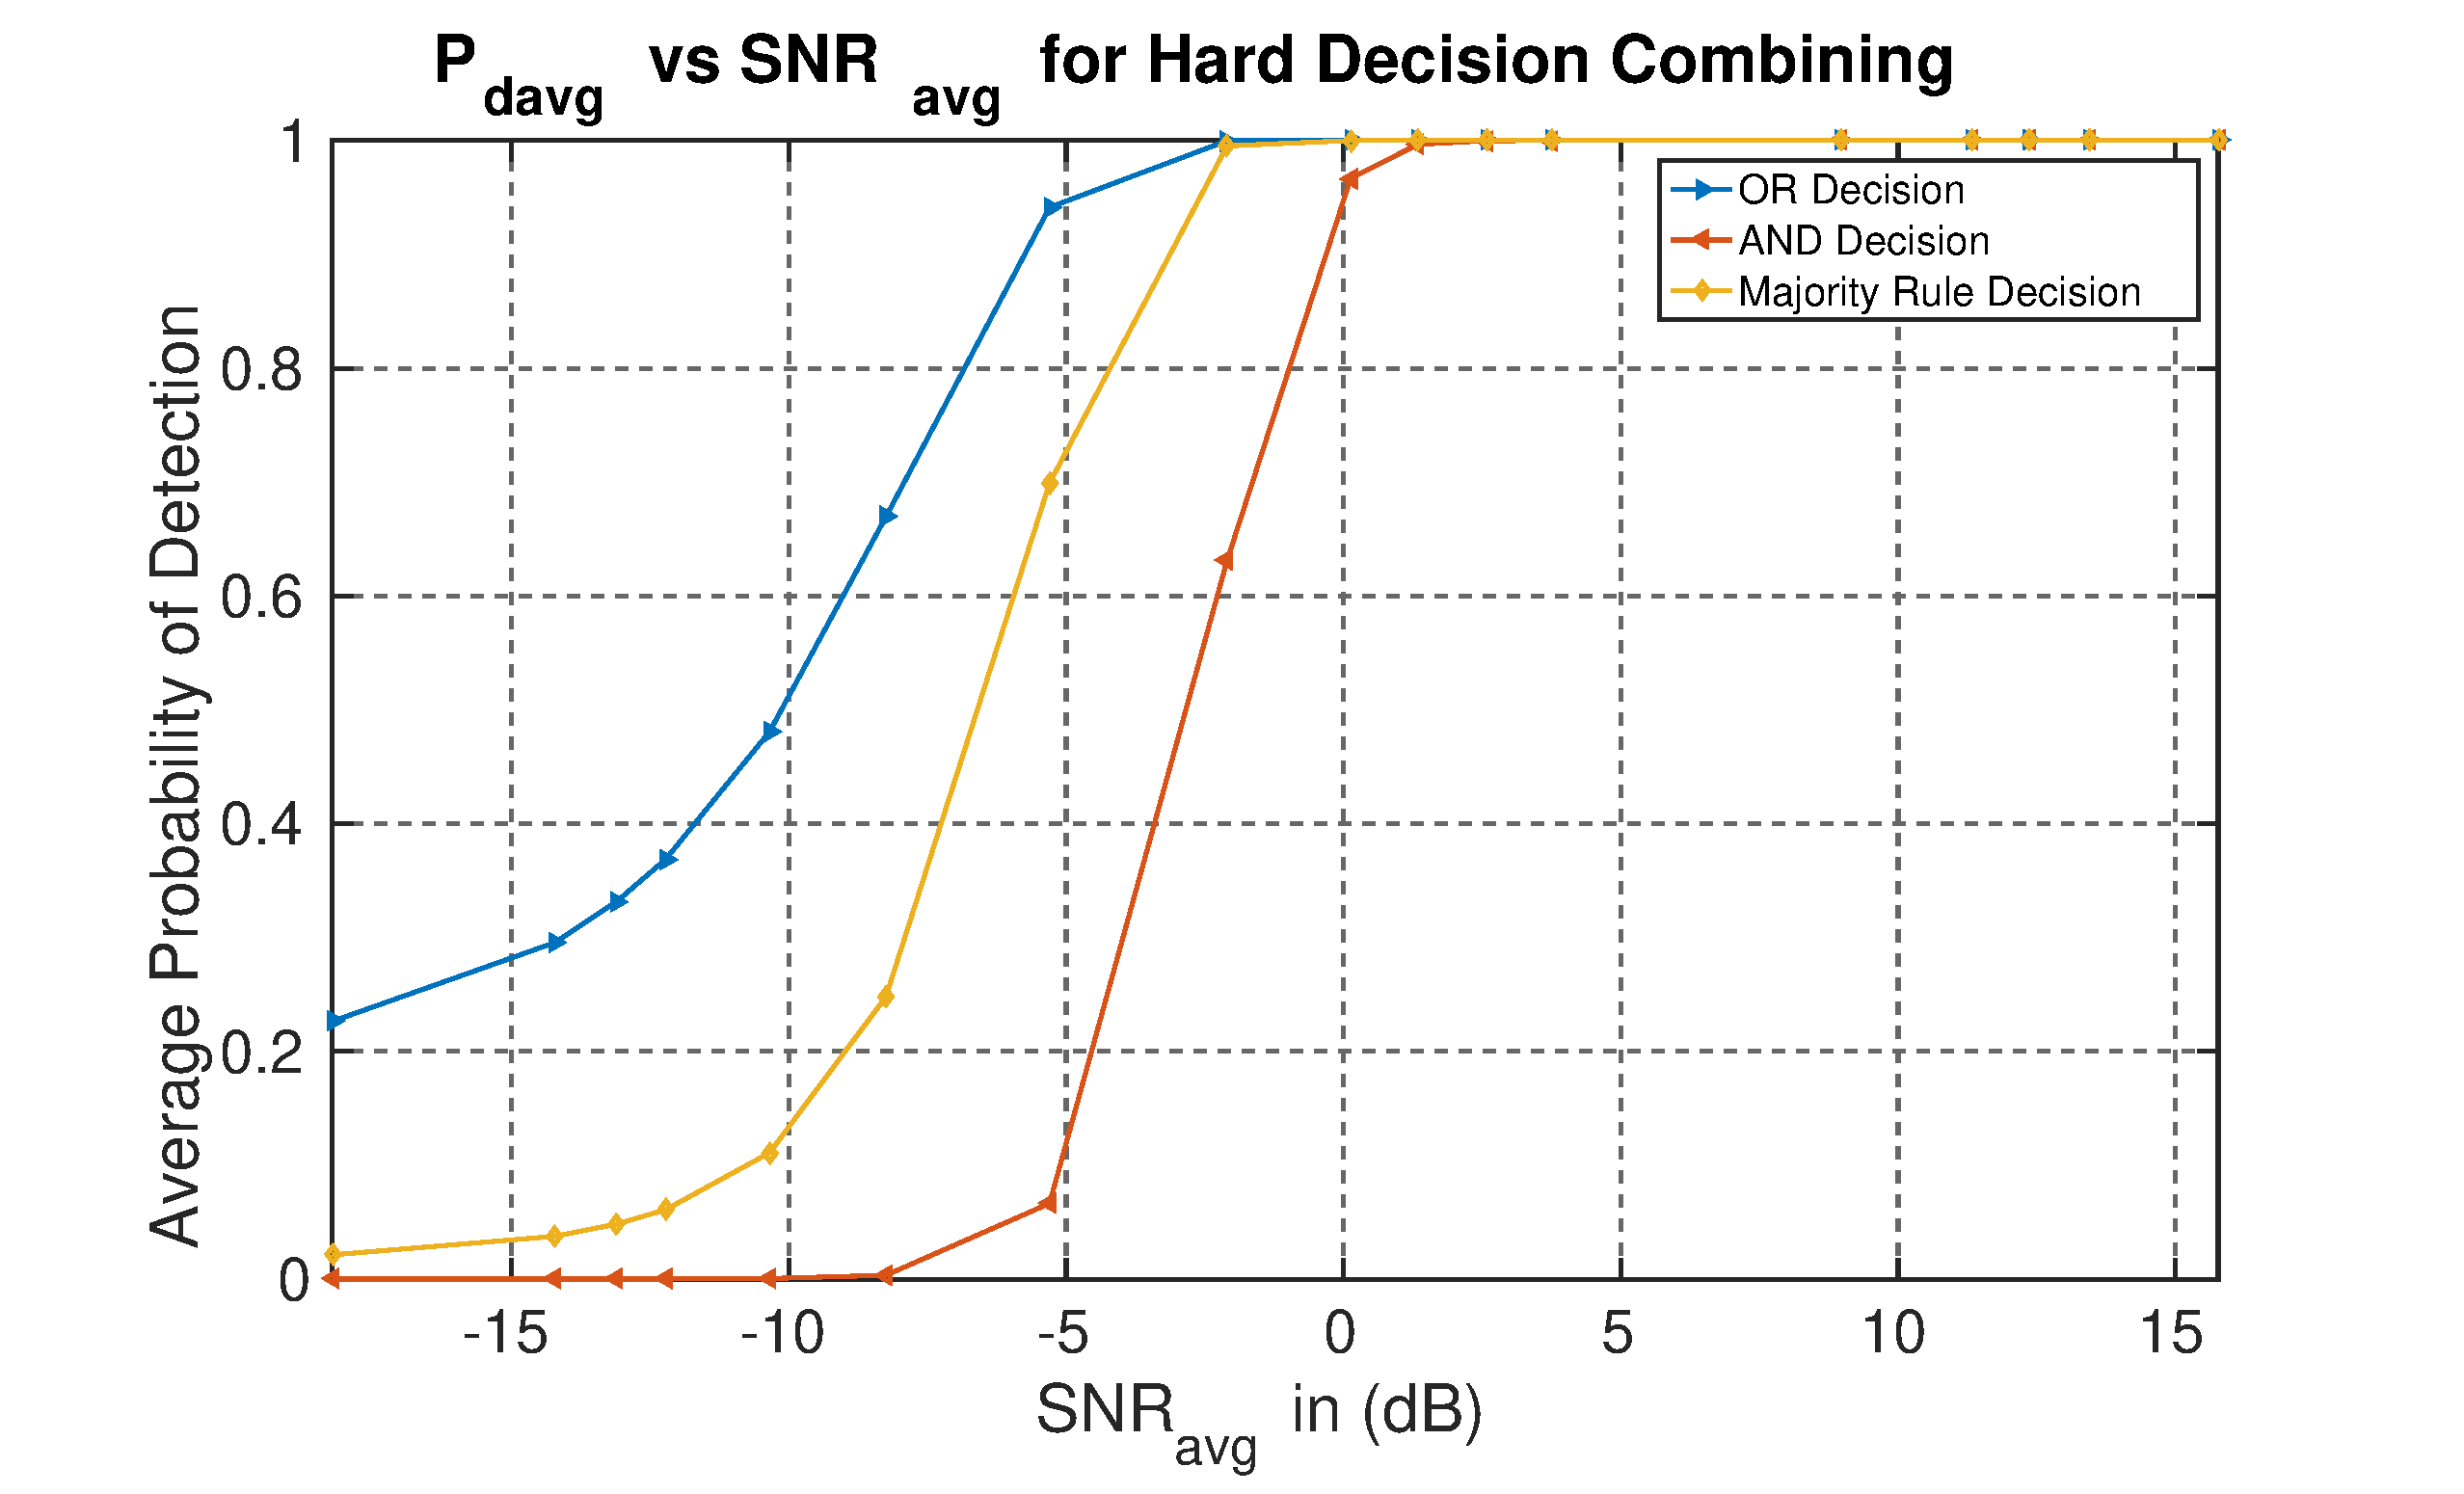
\includegraphics[width=\textwidth,keepaspectratio]{images/Gill/figs/hardecisionpd.eps}
    \caption{Probability of Detection versus $SNR_avg$ For Hard Decision Combining.} 
\label{hardres}      
\end{figure}

In Figure~\ref{hardroc}, the ROC characteristics for the hard decision combining at two different $SNR_{avg}$ for all three hard data fusion schemes are provided. It is pretty evident from the plot that the OR scheme performs better than both the AND and majority rule schemes. The AND scheme performs the worst because it depends on all sensor nodes to have same decision, which is very difficult in a real fading environment. For lower SNR values, OR outperform the majority rule by a large margin but as we go to higher SNR values their performance converges.

\begin{figure}[ht!]
	\centering
	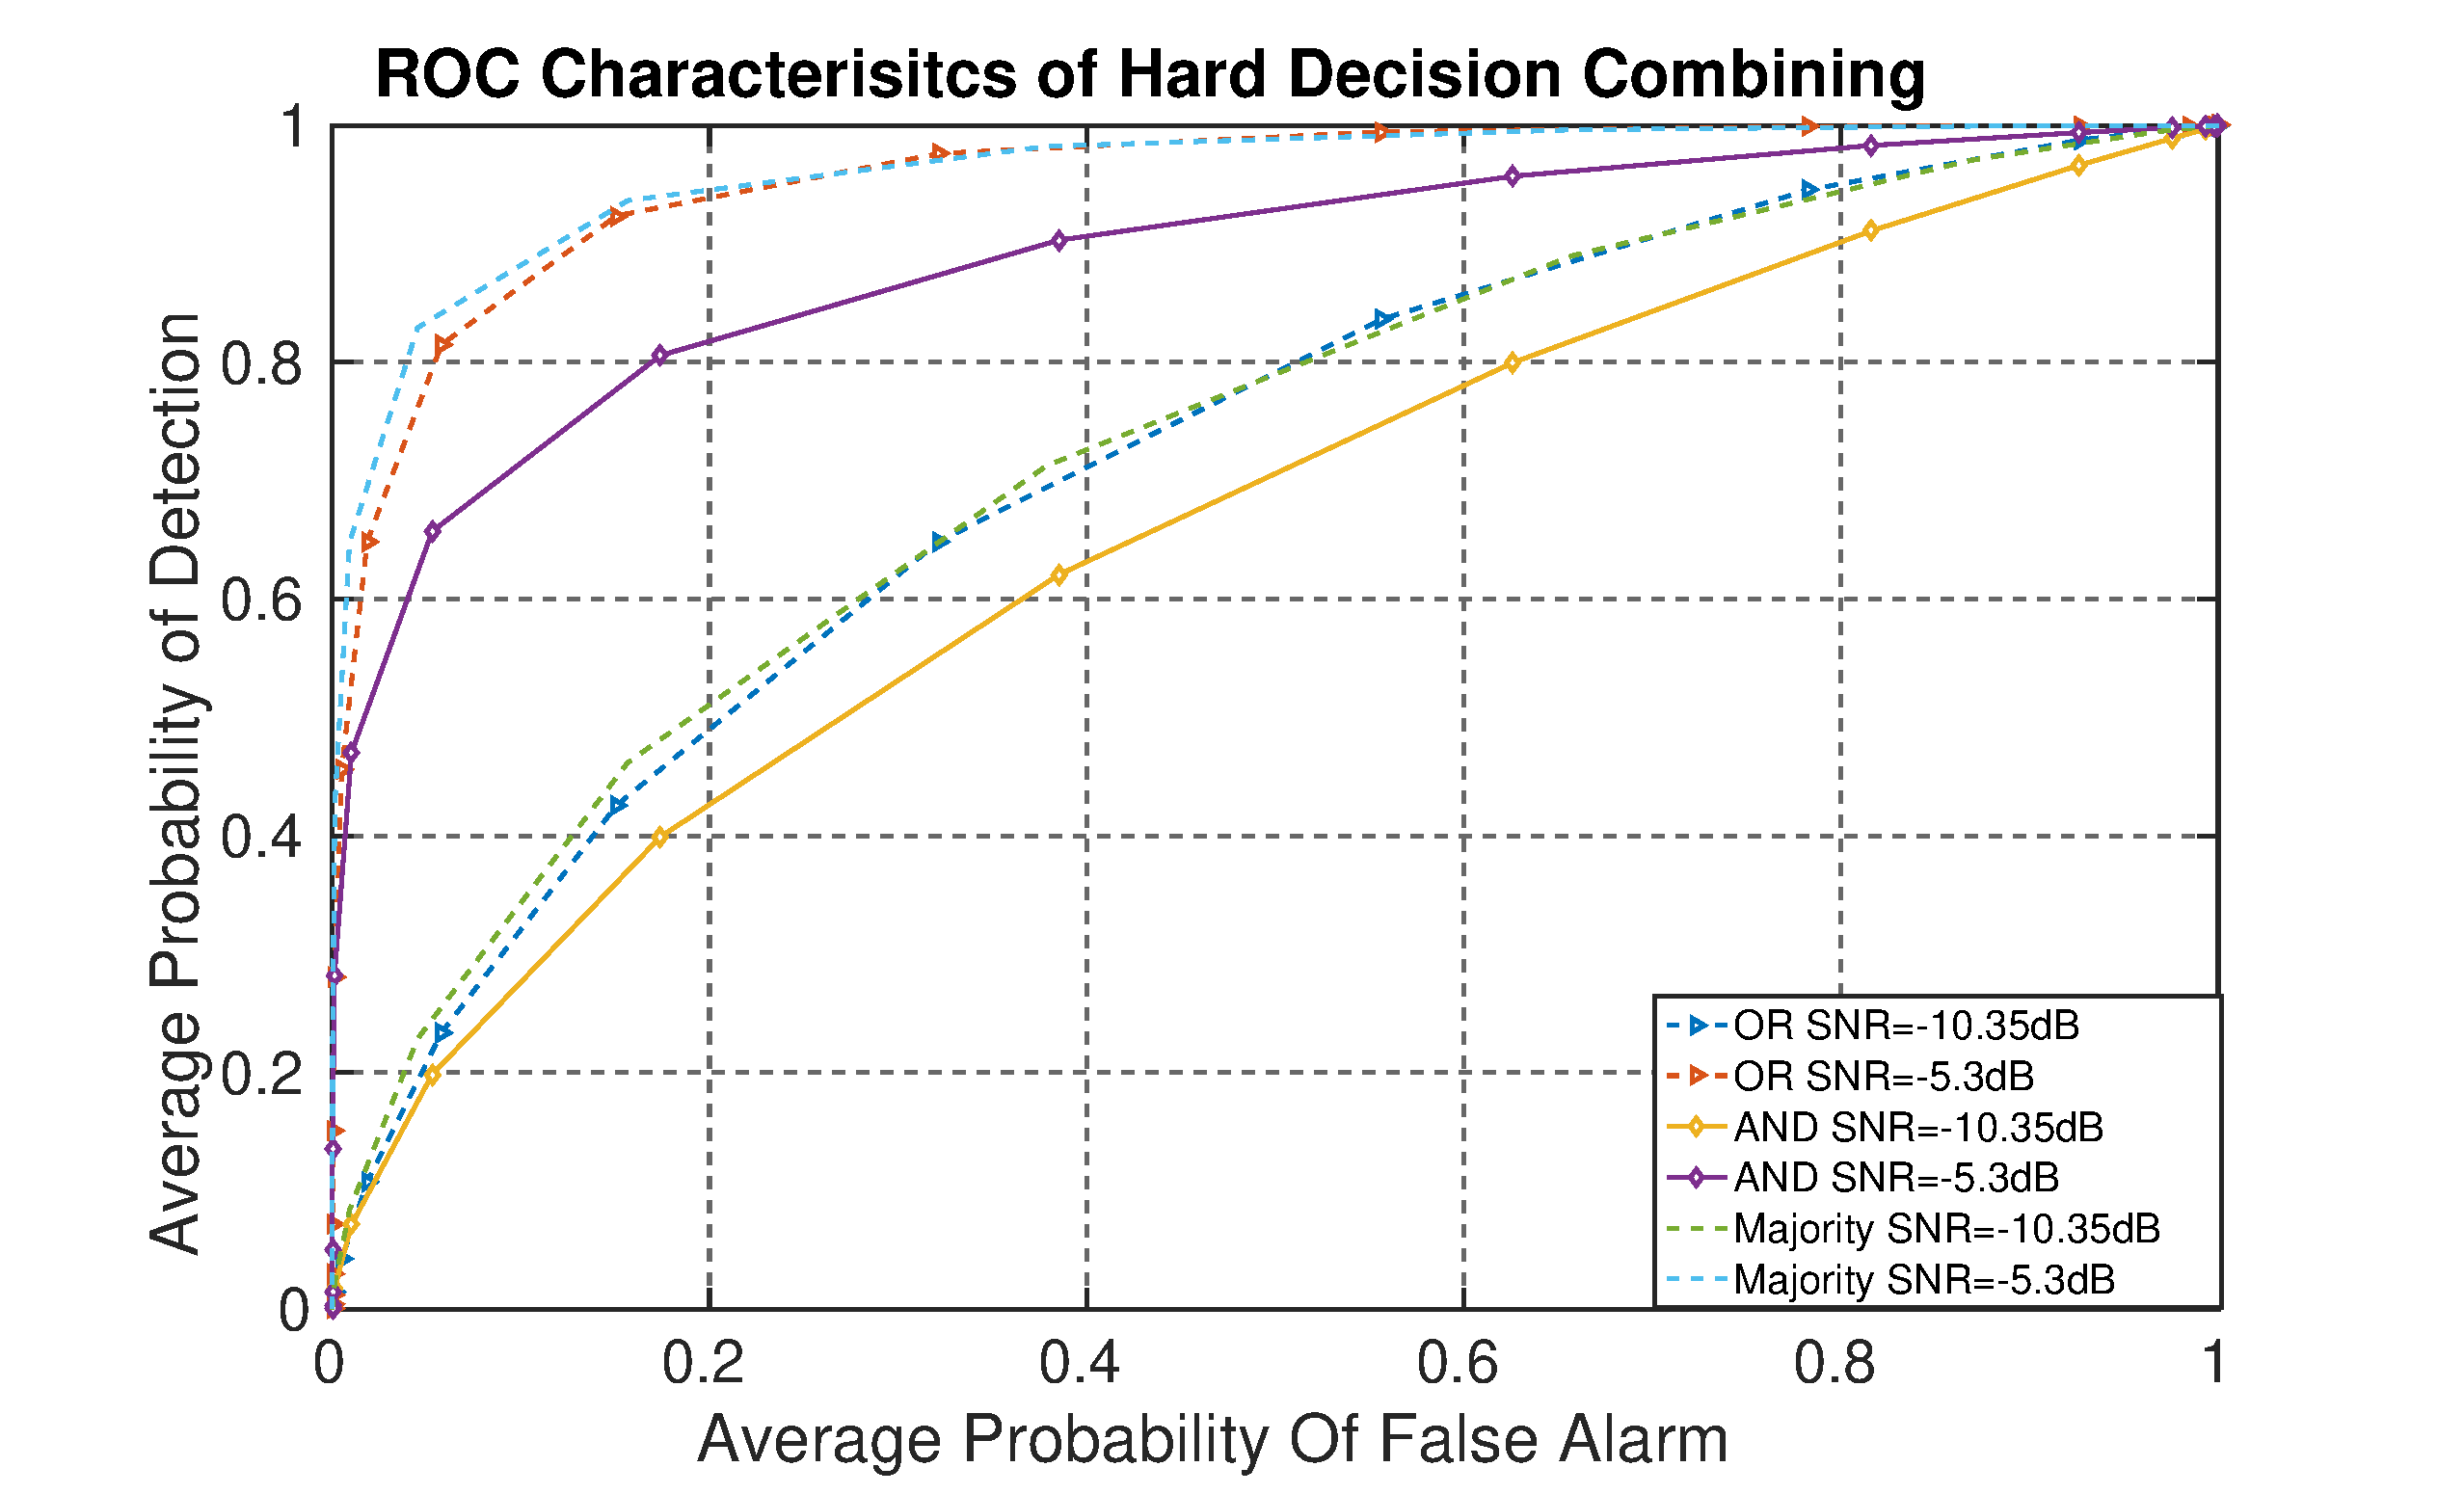
\includegraphics[width=\textwidth,keepaspectratio]{images/Gill/figs/hardecisioroc.eps}
    \caption{ROC Characteristics for Hard Decision Combining with Different SNRs.} 
\label{hardroc}      
\end{figure}

Figure~\ref{softpd} shows the $P_{davg}$ versus $SNR_{avg}$ for both soft and hard data fusion schemes. MNE and OR schemes overlap on the plot because in MNE scheme we take the maximum normalized energy and compare it the global test statistic, whereas for the OR scheme we estimate the signal source by either of sensor node decision. This makes both the scheme almost same and this is visible in the results. The EGC scheme performs the best since it takes into consideration all the sensor nodes and its global test statistic gives equal weight to all sensor nodes. The AND scheme performs the worst as expected. It is very important to understand that at higher SNR values, $SNR_{avg} > 2$ dB, we see all schemes converging to the same decisions. This tells us that in noiseless environment, we can choose hard fusion schemes because of their implementation complexity and we can select soft fusion in severe fading environment as they tend to be more accurate in these scenarios.
\begin{figure}[ht!]
	\centering
	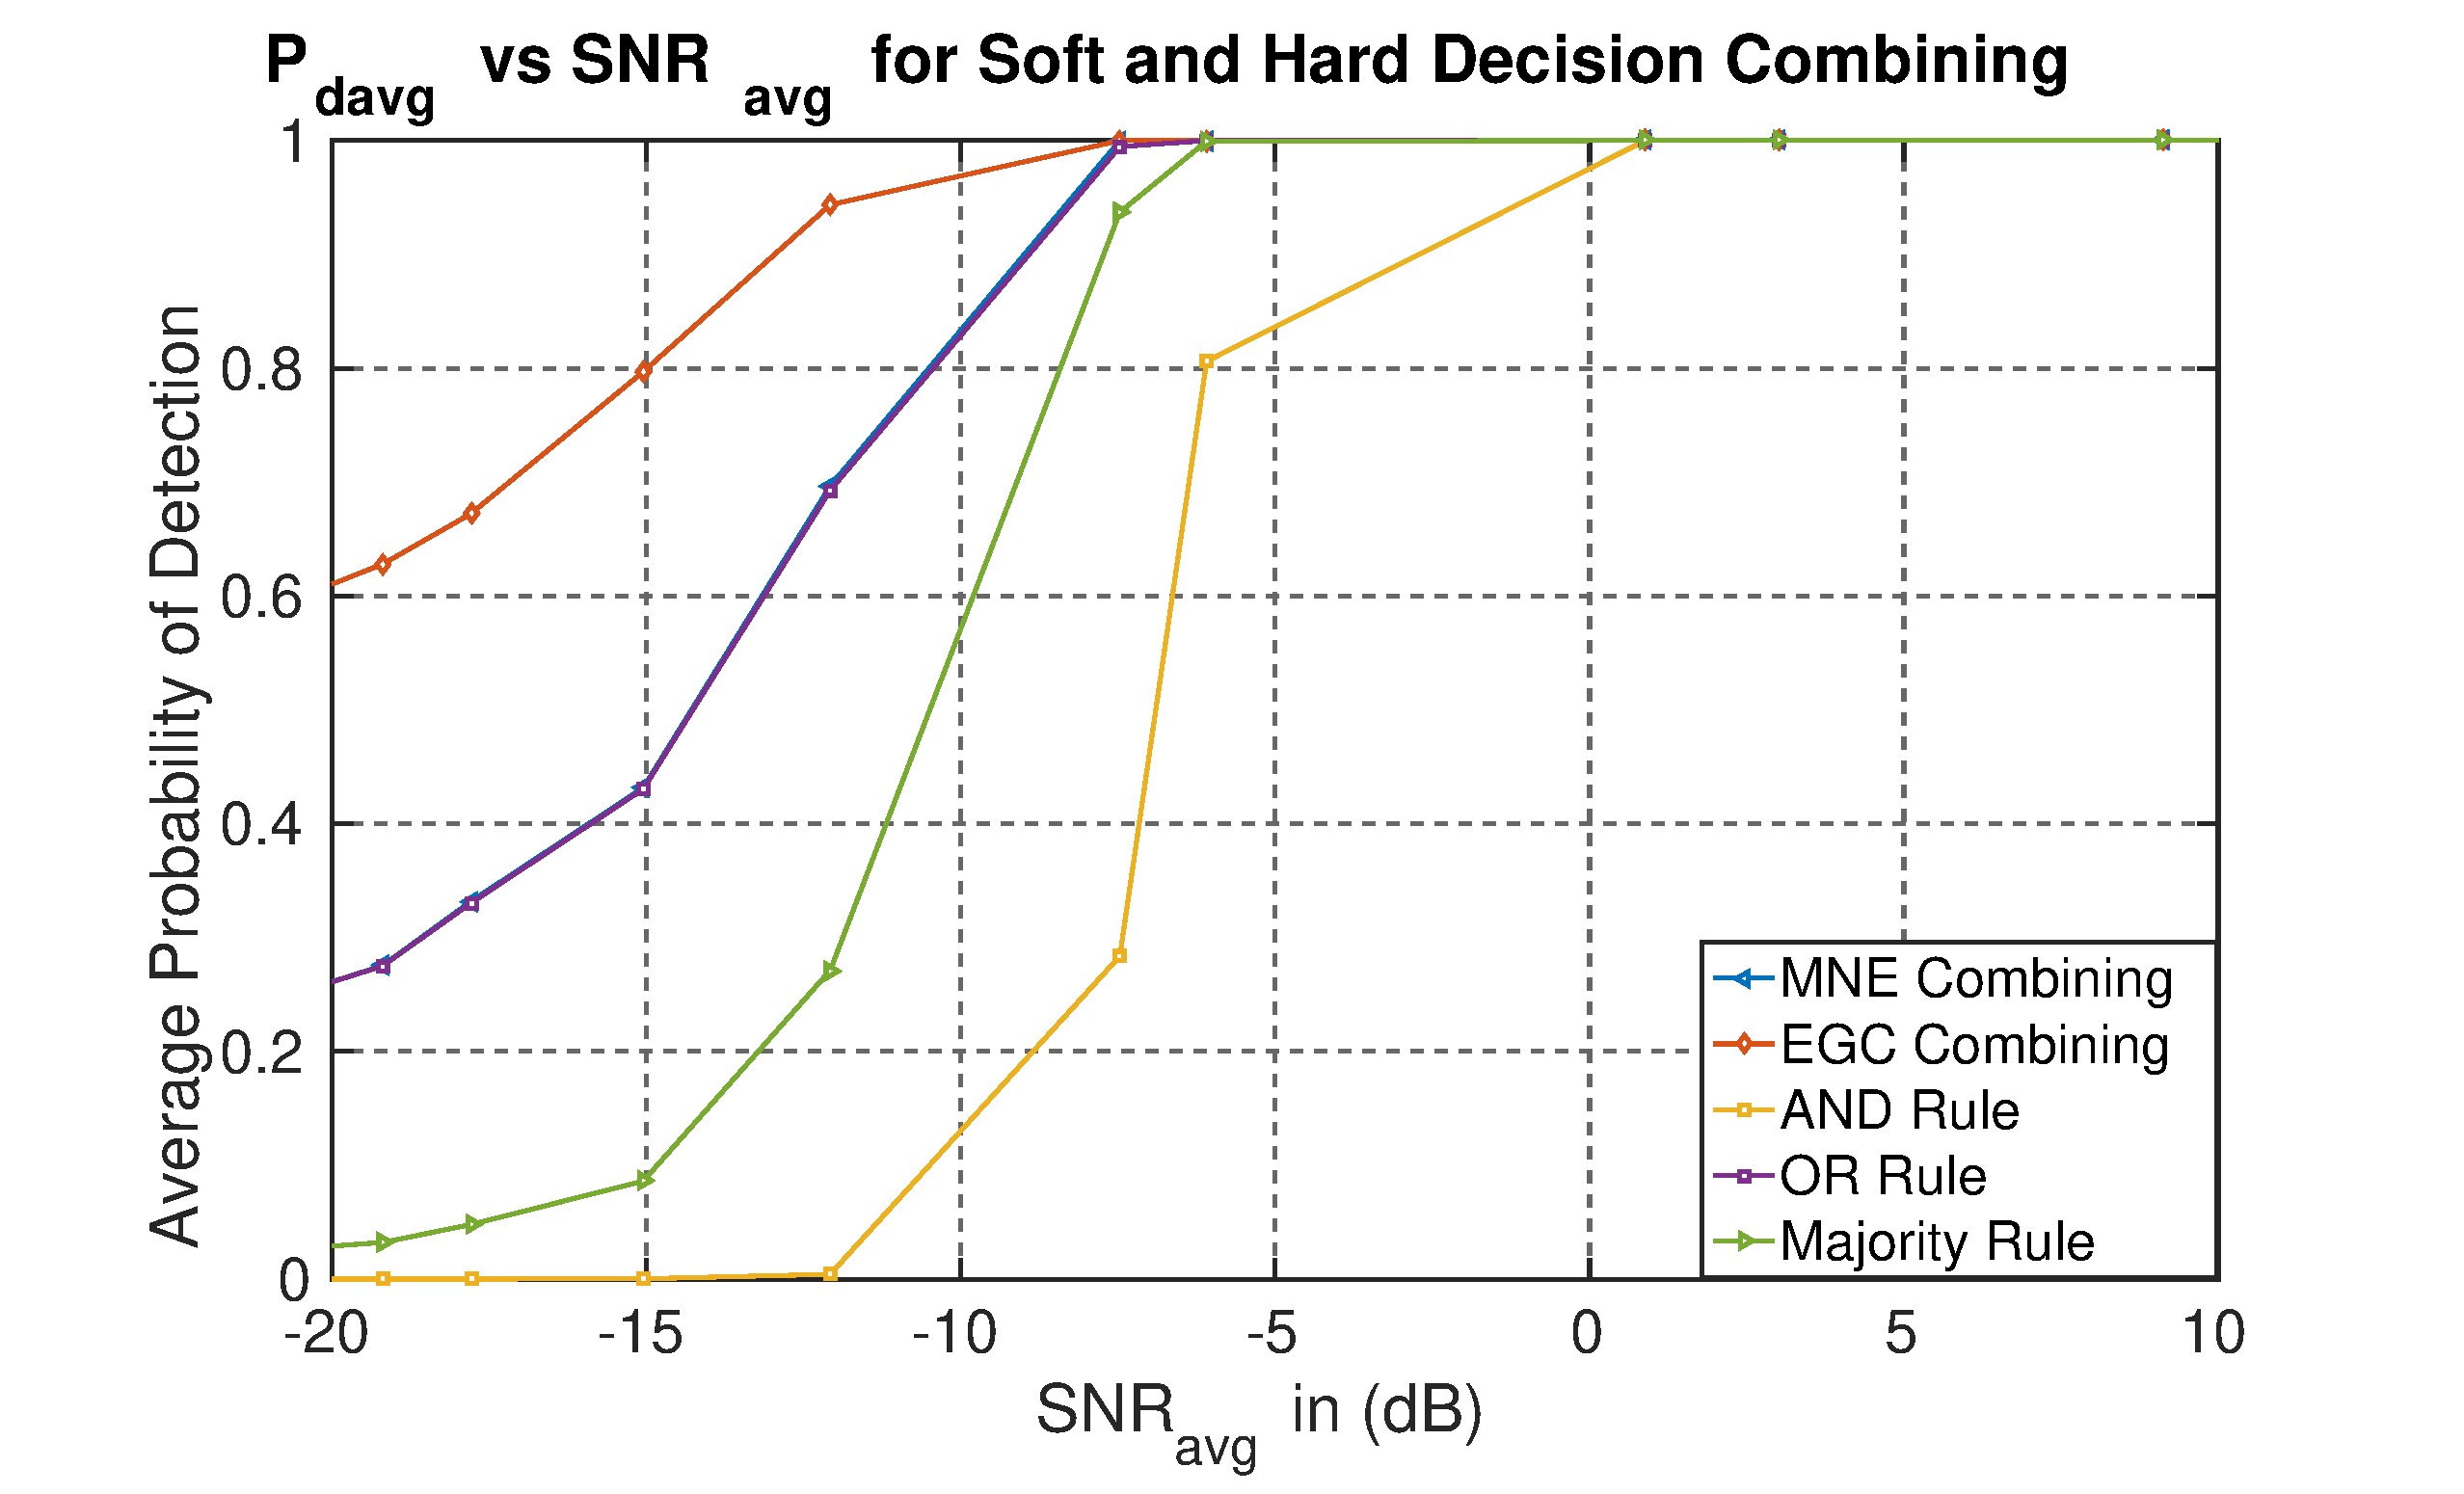
\includegraphics[width=\textwidth,keepaspectratio]{images/Gill/figs/softnhardecisionpd.eps}
    \caption{Probability of Detection versus $SNR_avg$ For Soft and Hard Decision Combining.} 
\label{softpd}      
\end{figure}

\section{Summary}
In this chapter, we described the test-bed setup using USRP N210 and RTL-SDR with different operating characteristics. The proposed heterogeneous CSS performance for both soft and hard data fusion approaches was derived at different SNR values. For soft-data fusion, scheme we use maximum normalized energy (MNE) and equal gain combining (EGC) scheme, and for hard data fusion scheme we used AND, OR and Majority Rule approaches. The results show that soft-data fusion scheme performs better than hard data fusion schemes for low SNR values, but as we increase SNR both schemes converges to same values. We learned that for severe environment, we can use soft-fusion and for noise-free environment hard decision schemes can be used due to their low implementation complexity.
